\documentclass[14pt]{extbook}
\usepackage{multicol, enumerate, enumitem, hyperref, color, soul, setspace, parskip, fancyhdr} %General Packages
\usepackage{amssymb, amsthm, amsmath, latexsym, units, mathtools} %Math Packages
\everymath{\displaystyle} %All math in Display Style
% Packages with additional options
\usepackage[headsep=0.5cm,headheight=12pt, left=1 in,right= 1 in,top= 1 in,bottom= 1 in]{geometry}
\usepackage[usenames,dvipsnames]{xcolor}
\usepackage{dashrule}  % Package to use the command below to create lines between items
\newcommand{\litem}[1]{\item#1\hspace*{-1cm}\rule{\textwidth}{0.4pt}}
\pagestyle{fancy}
\lhead{Module7}
\chead{}
\rhead{Version ALL}
\lfoot{5507-6544}
\cfoot{}
\rfoot{test}
\begin{document}

\begin{enumerate}
\item{
Solve the rational equation below.\[ \frac{6x}{-3x + 4} + \frac{-7x^{2}}{-6x^{2} -13 x + 28} = \frac{2}{2x + 7} \]} \newpage
\item{
Determine the domain of the function below.\[ f(x) = \frac{4}{25x^{2} -9} \]} \newpage
\item{
Solve the rational equation below.\[ \frac{3}{-9x -2} + -3 = \frac{-4}{81x + 18} \]} \newpage
\item{
Solve the rational equation below.\[ \frac{36}{24x -108} + 1 = \frac{36}{24x -108} \]} \newpage
\item{
Write an equation that can represent the function graphed below.
\begin{center}
    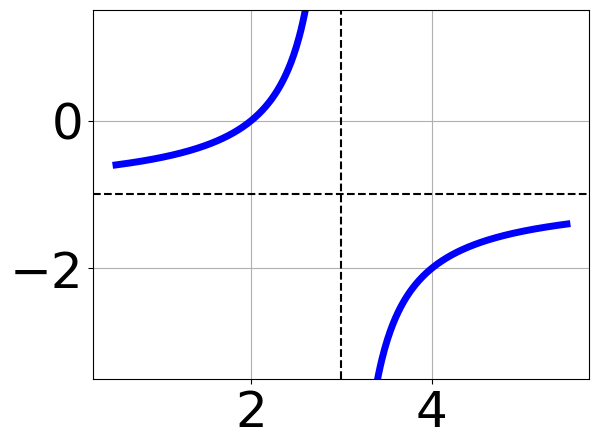
\includegraphics[width=0.5\textwidth]{../Figures/rationalGraphToEquationA.png}
\end{center}
} \newpage
\item{
Sketch a graph that represents the equation below.\[ f(x) = \frac{1}{(x - 1)^2} - 3 \]} \newpage
\item{
Determine the domain of the function below.\[ f(x) = \frac{5}{30x^{2} -30} \]} \newpage
\item{
Solve the rational equation below.\[ \frac{4x}{2x + 5} + \frac{-7x^{2}}{4x^{2} +16 x + 15} = \frac{3}{2x + 3} \]} \newpage
\item{
Write an equation that can represent the function graphed below.
\begin{center}
    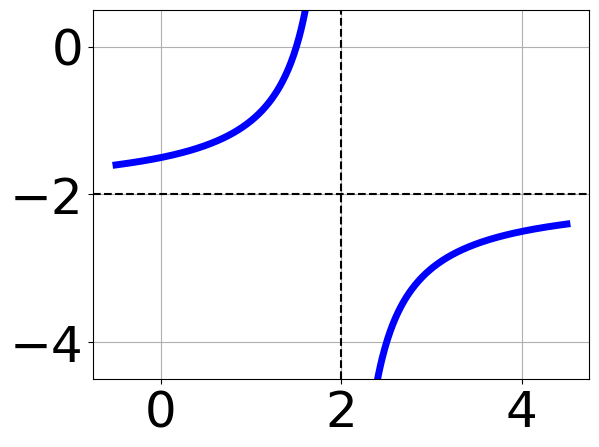
\includegraphics[width=0.5\textwidth]{../Figures/rationalGraphToEquationCopyA.png}
\end{center}
} \newpage
\item{
Sketch a graph that represents the equation below.\[ f(x) = \frac{1}{(x - 2)^2} + 1 \]} \newpage
\item{
Solve the rational equation below.\[ \frac{-4x}{-2x + 7} + \frac{-3x^{2}}{-14x^{2} +35 x + 49} = \frac{3}{7x + 7} \]} \newpage
\item{
Determine the domain of the function below.\[ f(x) = \frac{4}{25x^{2} -5 x -12} \]} \newpage
\item{
Solve the rational equation below.\[ \frac{3}{8x + 7} + 5 = \frac{3}{-32x -28} \]} \newpage
\item{
Solve the rational equation below.\[ \frac{-98}{-42x + 42} + 1 = \frac{-98}{-42x + 42} \]} \newpage
\item{
Write an equation that can represent the function graphed below.
\begin{center}
    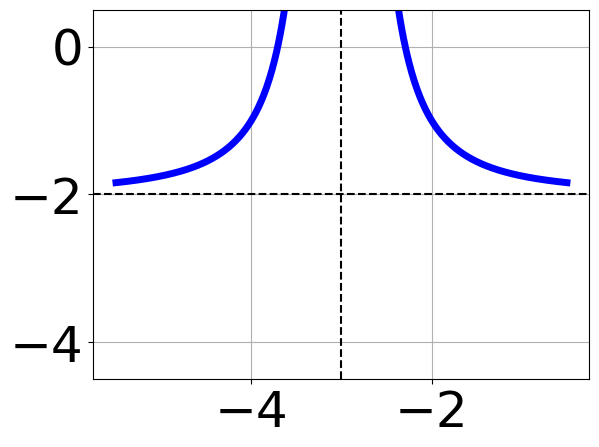
\includegraphics[width=0.5\textwidth]{../Figures/rationalGraphToEquationB.png}
\end{center}
} \newpage
\item{
Sketch a graph that represents the equation below.\[ f(x) = \frac{-1}{x + 1} - 3 \]} \newpage
\item{
Determine the domain of the function below.\[ f(x) = \frac{4}{9x^{2} -27 x + 20} \]} \newpage
\item{
Solve the rational equation below.\[ \frac{-2x}{-6x + 5} + \frac{-5x^{2}}{30x^{2} -43 x + 15} = \frac{-4}{-5x + 3} \]} \newpage
\item{
Write an equation that can represent the function graphed below.
\begin{center}
    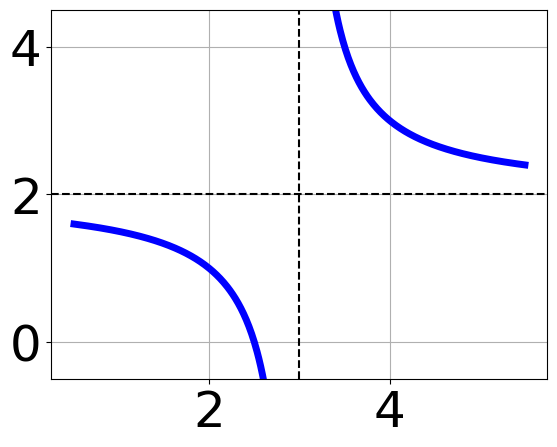
\includegraphics[width=0.5\textwidth]{../Figures/rationalGraphToEquationCopyB.png}
\end{center}
} \newpage
\item{
Sketch a graph that represents the equation below.\[ f(x) = \frac{1}{x - 2} - 3 \]} \newpage
\item{
Solve the rational equation below.\[ \frac{7x}{3x + 7} + \frac{-6x^{2}}{15x^{2} +44 x + 21} = \frac{-6}{5x + 3} \]} \newpage
\item{
Determine the domain of the function below.\[ f(x) = \frac{6}{15x^{2} +43 x + 30} \]} \newpage
\item{
Solve the rational equation below.\[ \frac{63}{-56x + 28} + 1 = \frac{63}{-56x + 28} \]} \newpage
\item{
Solve the rational equation below.\[ \frac{2}{-6x + 9} + 3 = \frac{4}{18x -27} \]} \newpage
\item{
Write an equation that can represent the function graphed below.
\begin{center}
    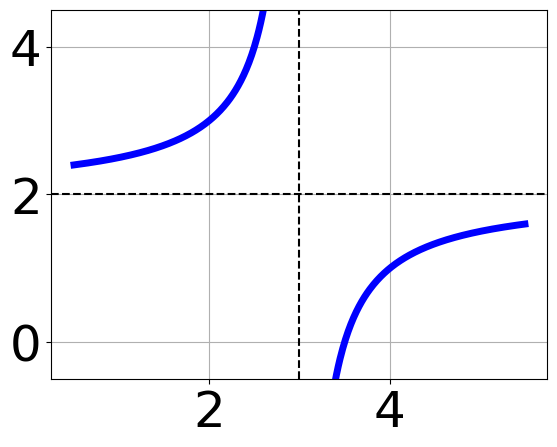
\includegraphics[width=0.5\textwidth]{../Figures/rationalGraphToEquationC.png}
\end{center}
} \newpage
\item{
Sketch a graph that represents the equation below.\[ f(x) = \frac{1}{(x - 1)^2} - 3 \]} \newpage
\item{
Determine the domain of the function below.\[ f(x) = \frac{3}{20x^{2} +3 x -9} \]} \newpage
\item{
Solve the rational equation below.\[ \frac{-5x}{-3x -5} + \frac{-4x^{2}}{-9x^{2} -24 x -15} = \frac{5}{3x + 3} \]} \newpage
\item{
Write an equation that can represent the function graphed below.
\begin{center}
    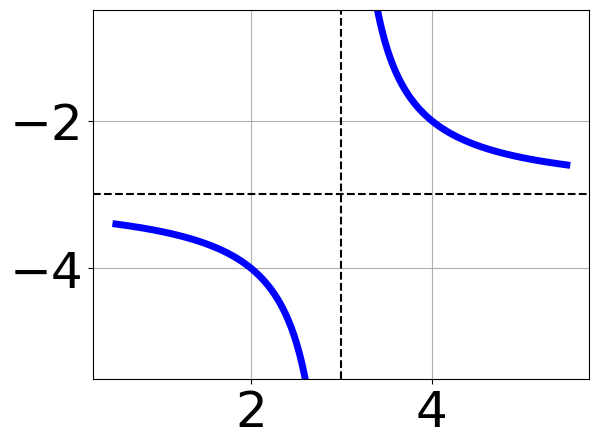
\includegraphics[width=0.5\textwidth]{../Figures/rationalGraphToEquationCopyC.png}
\end{center}
} \newpage
\item{
Sketch a graph that represents the equation below.\[ f(x) = \frac{-1}{x - 3} - 3 \]} \newpage
\end{enumerate}

\end{document}